\documentclass{article}
\usepackage[backend=biber]{biblatex}
\usepackage{graphicx}
\usepackage[]{hyperref}
\usepackage{graphicx}
\usepackage{svgcolor}
\usepackage{lscape}
\usepackage{booktabs}
\usepackage{longtable}
\usepackage{float}
\usepackage[table,xcdraw]{xcolor}
\usepackage{siunitx}
\usepackage[]{amsmath}
\usepackage{physics}
\usepackage{gensymb}
\usepackage{mathtools}
\usepackage{fancyref}
\addbibresource{/home/giorgio/Bibliography/bibliography.bib}
\hypersetup{
    colorlinks=true,
    linkcolor=blue,
    filecolor=magenta,      
    urlcolor=cyan,
    pdftitle={Relazione Veicoli Aerospaziali},
    bookmarks=true,
}
\author{Giorgio De Trane s275514}
\title{\textbf{RELAZIONE VEICOLI AEROSPAZIALI}}

\begin{document}

\maketitle
\begin{center}
    \textit{Anno accademico 2020-2021}
\end{center}
\begin{figure}[h!]
    \centering
    
\includegraphics[width=\textwidth]{Sources/Plots_and_Pictures/polito_logo.png}\\
\end{figure}
\pagebreak
\tableofcontents
\pagebreak
\section{Assignment 1\label{Assignment_1}}
\subsection{Assignment 1.1\label{Assignment_1.1}}

\textbf{Assignment}: Write down an initial list of requirements for an
aircraft that shall replace A350, with an entry into service in 2030.
Please, while listing the requirements, refer to the categories
reported in Sect.1.4
\newline
\newline
\textbf{\textit{List of Requirements}}\\\\ (Mainly based on Airbus A350-900 \autocite{Airbus_A350-900})
\\ 

\textbf{Design and Performance\label{Design_and_performance}}
\begin{itemize}
    \item Number of pilots: 2
    \item Cruise Mach: 0.85
    \item Max Operating Speed Mach: 0.9
    \item Cabin Crew: 8 (2 for each emergency exit)
    \item Number of passengers: 440
    \item Wing Span: under 70 m
    \item Fuselage Length: under 75 m
    \item Range: over 15000 km
    \item Height: under 18 m
    \item Wing Surface: 450 m²
    \item Max Payload: over 50 metric tonnes
    \item Number of engines: 2
\end{itemize}
\pagebreak
\textbf{Operational requirements\label{Operational_requirements}}
\begin{itemize}
    \item Cruise altitude: 10 - 13 km
    \item Turn around time: under 60 mins
    \item Takeoff distance: under 1 km
    \item Landing distance: under 2.5 km
    \item Rate of climb: 3000 ft/min (Initial climb)
    \item Ceiling: 13.15 km (FL431)
\end{itemize}

\textbf{Analysis of applicable regulations\label{Analysis_applicable_regulations}}
\begin{itemize}
    \item Number of exits: 8
    \item External noise (a terra a 5km di distanza) decollo: under 90 dB
    \item External noise (a terra a 5km di distanza) atterraggio: under 95 dB
    \item N max in condizioni operative: 2.5
    \item N min in condizioni operative: -1
\end{itemize}
\pagebreak
\subsection{Assignment 1.2\label{Assignment_1.2}}
\textbf{Assignment}: On the basis of the list of Requirements elicited
in the previous step, identify a good list of reference aircraft and
collect data to be used as meaningful statistical population.\\ \\ \\ 

Several commercial aicrafts from \textit{Airbus} and \textit{Boeing} have been chosen, with
the goal of having a statistical population to compare to in mind, as well as a reference list for 
inspiration with consolidated concept designs and technologies.\\
Acquiring all the data for the entire population was not easy, as their availability is scattered and varies from source
to source.\\
Despite the overall scarcity of clear, organized and transparent information, a significant amount of statistically meaningful
data has been acquired and ordered in the following landscape tables.\\ \\ 
A \textit{GNU/Octave} \autocite{Octave} (or Matlab) script that elaborates all the data has been written, with the goal
of easy readability in mind, as everything has been split into functions. \\
The script and its functions are publicly available in this works' \textit{GitHub} repository \autocite{Airbus_replacement_repo} (\textit{Code} directory) and 
licensed under the \textit{GNU GPL v3} license.\\ 
Bear in mind that Octave outputs all the plots at once when you run the whole script, while on Matlab
you may need to run each separate Section, as some versions overwrite \textit{figure()} when it's implemented
within a custom function.\\ 
This will of course depend on the Matlab version you're currently running.\\ The code itself is short and easy to read,
while also being full of step-by-step comments.


\newpage


\begin{landscape}
    \begin{table}[]
    \centering
    \resizebox{1.7\textwidth}{!}{%
    \begin{tabular}{@{}lccccccccccc@{}}
    \rowcolor[HTML]{FF7A7A} 
    \cellcolor[HTML]{FFC99B}Design \& Performance parameters &
      \multicolumn{1}{l}{\cellcolor[HTML]{FF7A7A}B787-10 Dre} &
      \multicolumn{1}{l}{\cellcolor[HTML]{FF2C2C}A350 XWB-900} &
      \multicolumn{1}{l}{\cellcolor[HTML]{FF7A7A}A330 Neo -900} &
      \multicolumn{1}{l}{\cellcolor[HTML]{FF7A7A}B777-300ER} &
      \multicolumn{1}{l}{\cellcolor[HTML]{FF7A7A}B777 X-900} &
      \multicolumn{1}{l}{\cellcolor[HTML]{FF7A7A}B787-8} &
      \multicolumn{1}{l}{\cellcolor[HTML]{FF7A7A}A340-500} &
      \multicolumn{1}{l}{\cellcolor[HTML]{FF7A7A}A330-300} &
      \multicolumn{1}{l}{\cellcolor[HTML]{FF7A7A}A340-600} &
      \multicolumn{1}{l}{\cellcolor[HTML]{FF7A7A}A330-200} &
      \multicolumn{1}{l}{\cellcolor[HTML]{FF7A7A}B767-300} \\
    \rowcolor[HTML]{EFEFEF} 
    \cellcolor[HTML]{FFEF98}Number of pilots                & 2     & 2     & 2     & 2     & 2     & 2      & 2     & 2     & N.A.  & 2    & 2    \\
    \cellcolor[HTML]{FCF1B3}Cruise Mach number              & 0.85  & 0.85  & 0.81  & 0.84  & 0.84  & 0.85   & 0.83  & 0.86  & N.A.  & 0.86 & 0.86 \\
    \rowcolor[HTML]{EFEFEF} 
    \cellcolor[HTML]{FFEF98}Max Operating Speed Mach        & N.A.  & N.A.  & N.A.  & N.A.  & N.A.  & N.A.   & N.A.  & N.A.  & N.A.  & N.A. & N.A. \\
    \cellcolor[HTML]{FCF1B3}Cabin Crew                      & 8-9   & 8-9   & 8-9   & 14    & N.A.  & N.A.   & N.A.  & N.A.  & N.A.  & N.A. & N.A. \\
    \rowcolor[HTML]{EFEFEF} 
    \cellcolor[HTML]{FFEF98}Number of passengers            & 330   & 440   & 440   & 550   & 426   & 359    & 375   & 275   & N.A.  & N.A. & N.A. \\
    \cellcolor[HTML]{FCF1B3}Wing Span {[}m²{]}              & 60.81 & 64.75 & 64    & 64.8  & 72.8  & 60.12  & 60.3  & N.A.  & N.A.  & N.A. & N.A. \\
    \rowcolor[HTML]{EFEFEF} 
    \cellcolor[HTML]{FFEF98}Fuselage Length {[}m{]}         & 68    & 66.8  & 63.66 & 73.86 & 76.72 & 56.72  & 67.93 & N.A.  & N.A.  & N.A. & N.A. \\
    \cellcolor[HTML]{FCF1B3}Range {[}km{]}                  & 11750 & 15000 & 13334 & 13650 & 13500 & 13620  & 12400 & 11750 & 14450 & N.A. & N.A. \\
    \rowcolor[HTML]{EFEFEF} 
    \cellcolor[HTML]{FFEF98}Wing Surface {[}m²{]}           & 377   & 443   & 465   & 436.8 & 516.7 & 377    & 437.3 & N.A.  & N.A.  & N.A. & N.A. \\
    \cellcolor[HTML]{FCF1B3}Height {[}m{]}                  & 17.02 & 17.47 & 16.79 & 18.76 & 19.53 & 16.92  & 17.53 & N.A.  & N.A.  & N.A. & N.A. \\
    \rowcolor[HTML]{EFEFEF} 
    \cellcolor[HTML]{FFEF98}Max Payload {[}metric tonnes{]} & 57    & 53    & 44    & 69.8  & 73.5  & 43.318 & 54    & N.A.  & N.A.  & N.A. & N.A. \\
    \cellcolor[HTML]{FCF1B3}Number of engines               & 2     & 2     & 2     & 2     & 2     & 2      & 4     & N.A.  & N.A.  & N.A. & N.A.
    \end{tabular}%
    }
    \caption{Statistical Population - Design and Performance parameters}
    \label{tab:stat_pop_des_perf}
    \end{table}
\end{landscape}

    \clearpage
    \newpage

\begin{landscape}
    \begin{table}[]
    \centering
    \resizebox{1.7\textwidth}{!}{%
    \begin{tabular}{@{}lccccccccccc@{}}
    \rowcolor[HTML]{FF7A7A} 
    \cellcolor[HTML]{FFC99B}Operational requirements &
      \multicolumn{1}{l}{\cellcolor[HTML]{FF7A7A}B787-10 Dre} &
      \multicolumn{1}{l}{\cellcolor[HTML]{FF2C2C}A350 XWB-900} &
      \multicolumn{1}{l}{\cellcolor[HTML]{FF7A7A}A330 Neo -900} &
      \multicolumn{1}{l}{\cellcolor[HTML]{FF7A7A}B777-300ER} &
      \multicolumn{1}{l}{\cellcolor[HTML]{FF7A7A}B777 X-900} &
      \multicolumn{1}{l}{\cellcolor[HTML]{FF7A7A}B787-8} &
      \multicolumn{1}{l}{\cellcolor[HTML]{FF7A7A}A340-500} &
      \multicolumn{1}{l}{\cellcolor[HTML]{FF7A7A}A330-300} &
      \multicolumn{1}{l}{\cellcolor[HTML]{FF7A7A}A340-600} &
      \multicolumn{1}{l}{\cellcolor[HTML]{FF7A7A}A330-200} &
      \multicolumn{1}{l}{\cellcolor[HTML]{FF7A7A}B767-300} \\
    \rowcolor[HTML]{EFEFEF} 
    \cellcolor[HTML]{FFEF98}Cruise altitude {[}m{]}    & N.A.  & N.A.   & N.A.  & N.A.  & 13136.88 & N.A.  & N.A.  & N.A. & N.A. & N.A. & N.A. \\
    \cellcolor[HTML]{FCF1B3}Turn around time {[}min{]} & 44    & 34 -62 & N.A.  & 30    & N.A.     & N.A.  & N.A.  & N.A. & N.A. & N.A. & N.A. \\
    \rowcolor[HTML]{EFEFEF} 
    \cellcolor[HTML]{FFEF98}Takeoff distance {[}m{]}   & 2600  & N.A.   & N.A.  & N.A.  & N.A.     & 2600  & 13350 & N.A. & N.A. & N.A. & N.A. \\
    \cellcolor[HTML]{FCF1B3}Landing distance {[}m{]}   & 2000  & N.A.   & N.A.  & N.A.  & N.A.     & N.A.  & N.A.  & N.A. & N.A. & N.A. & N.A. \\
    \rowcolor[HTML]{EFEFEF} 
    \cellcolor[HTML]{FFEF98}Rate of climb              & N.A.  & N.A.   & N.A.  & N.A.  & N.A.     & N.A.  & N.A.  & N.A. & N.A. & N.A. & N.A. \\
    \cellcolor[HTML]{FCF1B3}Ceiling {[}m{]}            & 13136 & 13100  & 12634 & 13136 & 13140    & 13100 & 12634 & N.A. & N.A. & N.A. & N.A.
    \end{tabular}%
    }
    \caption{Statistical Population - Operational Requirements}
    \label{tab:stat_pop_op_req}
    \end{table}
    \end{landscape}
    \clearpage


\begin{landscape}
    \begin{table}[]
    \centering
    \resizebox{1.7\textwidth}{!}{%
    \begin{tabular}{@{}lccccccccccc@{}}
    \rowcolor[HTML]{FF7A7A} 
    \cellcolor[HTML]{FFC99B}\textbf{Weights, Fuel and Aerodynamics} &
      \multicolumn{1}{l}{\cellcolor[HTML]{FF7A7A}B787-10 Dre} &
      \multicolumn{1}{l}{\cellcolor[HTML]{FF2C2C}A350 XWB-900} &
      \multicolumn{1}{l}{\cellcolor[HTML]{FF7A7A}A330 Neo -900} &
      \multicolumn{1}{l}{\cellcolor[HTML]{FF7A7A}B777-300ER} &
      \multicolumn{1}{l}{\cellcolor[HTML]{FF7A7A}B777 X-900} &
      \multicolumn{1}{l}{\cellcolor[HTML]{FF7A7A}B787-8} &
      \multicolumn{1}{l}{\cellcolor[HTML]{FF7A7A}A340-500} &
      \multicolumn{1}{l}{\cellcolor[HTML]{FF7A7A}A330-300} &
      \multicolumn{1}{l}{\cellcolor[HTML]{FF7A7A}A340-600} &
      \multicolumn{1}{l}{\cellcolor[HTML]{FF7A7A}A330-200} &
      \multicolumn{1}{l}{\cellcolor[HTML]{FF7A7A}B767-300} \\
    \rowcolor[HTML]{EFEFEF} 
    \cellcolor[HTML]{FFEF98}MTOW {[}kg{]}           & 250000 & 275000 & 251000 & 351535 & 352000 & 227940 & 365000 & 242000 & 380000 & 230000 & 158758 \\
    \cellcolor[HTML]{FCF1B3}Fuel Mass {[}kg{]}      & 101456 & 110523 & 111272 & 146839 & 160000 & 101323 & 110400 & N.A.   & N.A.   & N.A.   & N.A.   \\
    \rowcolor[HTML]{EFEFEF} 
    \cellcolor[HTML]{FFEF98}Empty Weight {[}kg{]}   & 135500 & 142400 & 137000 & 167829 & 181400 & 119950 & 177755 & 109400 & 174000 & 120600 & 86069  \\
    \cellcolor[HTML]{FCF1B3}Allungamento Alare      & 10.03  & 9.49   & 11     & 9.82   & 9.96   & 9.59   & 9.3    & N.A.   & N.A.   & N.A.   & N.A.   \\
    \rowcolor[HTML]{EFEFEF} 
    \cellcolor[HTML]{FFEF98}Cruise Speed {[}km/h{]} & 1050   & 903    & 918    & 905    & 900    & 903    & 871    & N.A.   & N.A.   & N.A.   & N.A.   \\
    \cellcolor[HTML]{FCF1B3}L/D                     & 20     & 21     & N.A.   & N.A.   & N.A.   & 21.23  & 16.2   & N.A.   & N.A.   & N.A.   & N.A.   \\
    \rowcolor[HTML]{EFEFEF} 
    \cellcolor[HTML]{FFEF98}SFC {[}lb/lbh{]}        & 0.506  & 0.478  & 0.506  & 0.56   & 0.545  & N.A.   & N.A.   & N.A.   & N.A.   & N.A.   & N.A.  
    \end{tabular}%
    }
    \caption{Statistical Population - Weights, Fuel and Aerodynamics}
    \label{tab:stat_pop_weight}
    \end{table}
    \end{landscape}
    \clearpage

\subsection{Assignment 1.3\label{Assignment_1.3}}
\textbf{Assignment}: \textit{Critical Analysis of statistical trends}.
Verify whether your statistical population fits the trend reported in
literature (e.g. Raymer) or suggest improvements to the simple
mathematical models (e.g. updates of coefficients).\\ \\ \\ 

Among all of the acquired data, the \textit{Empty Mass Fraction} is a particularly significant
statistical trend. \\
The raw data trend has been comparatively plot in the script, along with an improved algorithm, 
proposed by \textit{Daniel P. Raymer} \autocite{Raymer_Daniel}.

\begin{figure}[h!]
    \phantomsection
    \centering
    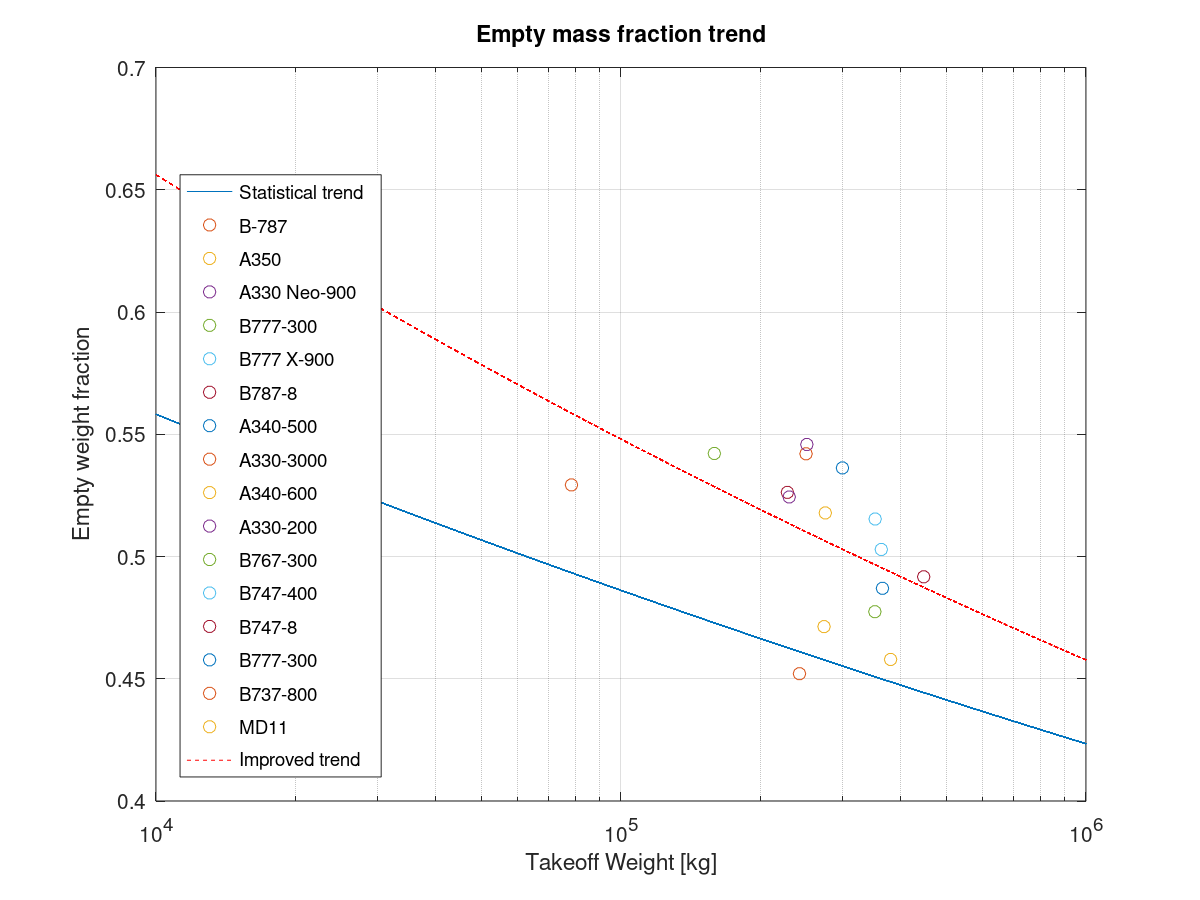
\includegraphics[width=\textwidth]{Sources/Plots_and_Pictures/Empty_mass_trend.png}\\
    \label{Empty_mass_trend}
    \caption{\textit{Empty Mass Trend}}
\end{figure} 

As clearly visible, the improved trend is substantially more in line with the acquired data.


\pagebreak
\subsection{Assignment 1.4\label{Assignments_1.4}}
\textbf{Assignment}: \textit{Guess data estimation for the reference
case study}. Apply the original or improved statistical trends to
perform the first guess data estimation for the reference case
study. Please, report all iterations needed to converge to the
design maximum take-off mass.\\ \\ \\ 

The first hypothesis for the \textit{MTOW} estimation was using the \textit{True Air Speed}
at an altitude of 10 km, as that would be a worse case scenario compared to the goal design
of a cruise Mach of 0.85. \\ 
The entire calculation is made assuming a range of 11 km and a maximum range of 15 km, as well as
a 50 metric tonnes design payload, with the awareness that a lighter payload might be necessary
in order to improve range.\\ \\
The function \begin{verbatim} mtow_range_plotter.m \end{verbatim} takes a guess \textit{MTOW} value as one of its inputs, generates some mass coefficients,
elaborates and uses them to finally return the desired \textit{MTOW} as one of its outputs (see repository \autocite{Airbus_replacement_repo} for the implementation).\\ 
The function also plots the MTOW as a function of the range.\\
One issue that has been immediately noticed is an instability with the plot around 15000 km,
therefore a compromise payload of 40 metric tonnes has been used for this specific plot, in order to 
get a more accurate visualization. \\ 
\begin{figure}[h!]
    \centering
    \phantomsection
    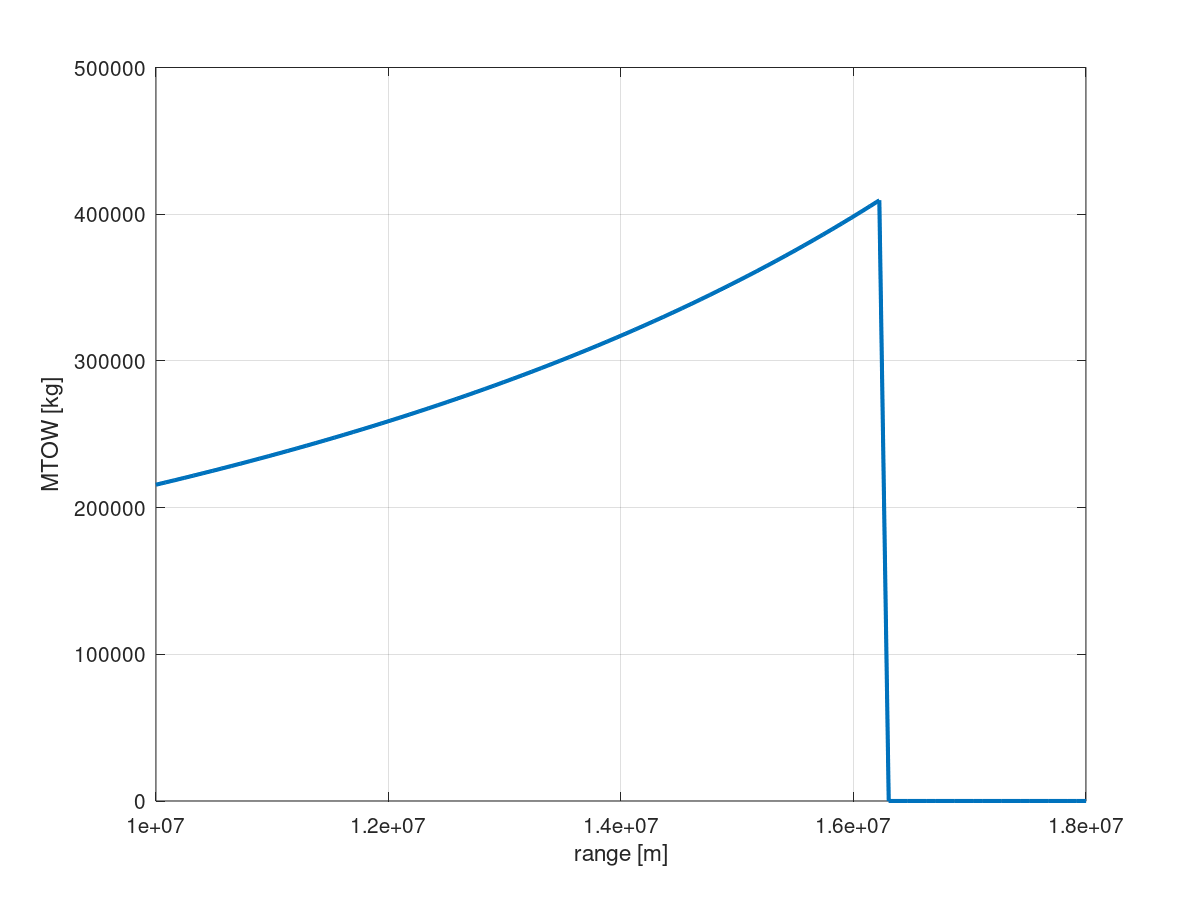
\includegraphics[width=0.7\textwidth]{Sources/Plots_and_Pictures/MTOW_range.png}
    \label{MTOW_Range}
    \caption{MTOW-Range}
\end{figure}
\clearpage
Similarly, with the function \autocite{Airbus_replacement_repo}
\begin{verbatim}

    mtow_payload_plotter.m

\end{verbatim}
the \textit{MTOW} has been plotted as a function of the payload with the design
range of 11000 km first, then with the maximum range of 15000 km, as pictured below.

\begin{figure}[h!]
    \centering
    \phantomsection
    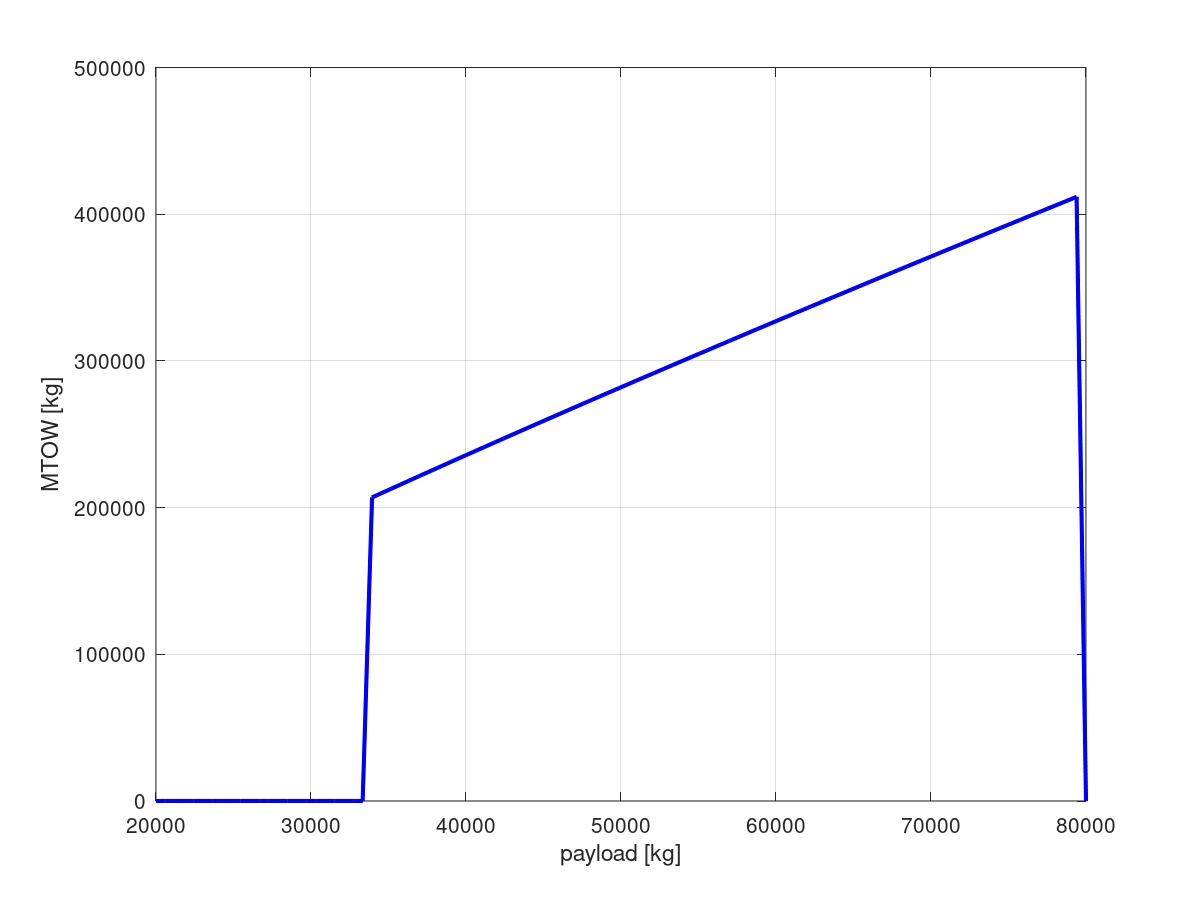
\includegraphics[width=\textwidth]{Sources/Plots_and_Pictures/MTOW_payload.png}
    \label{MTOW_Payload_11}
    \caption{MTOW-Payload (11000 km)}
\end{figure}
\clearpage
\begin{figure}[h!]
    \centering
    \phantomsection
    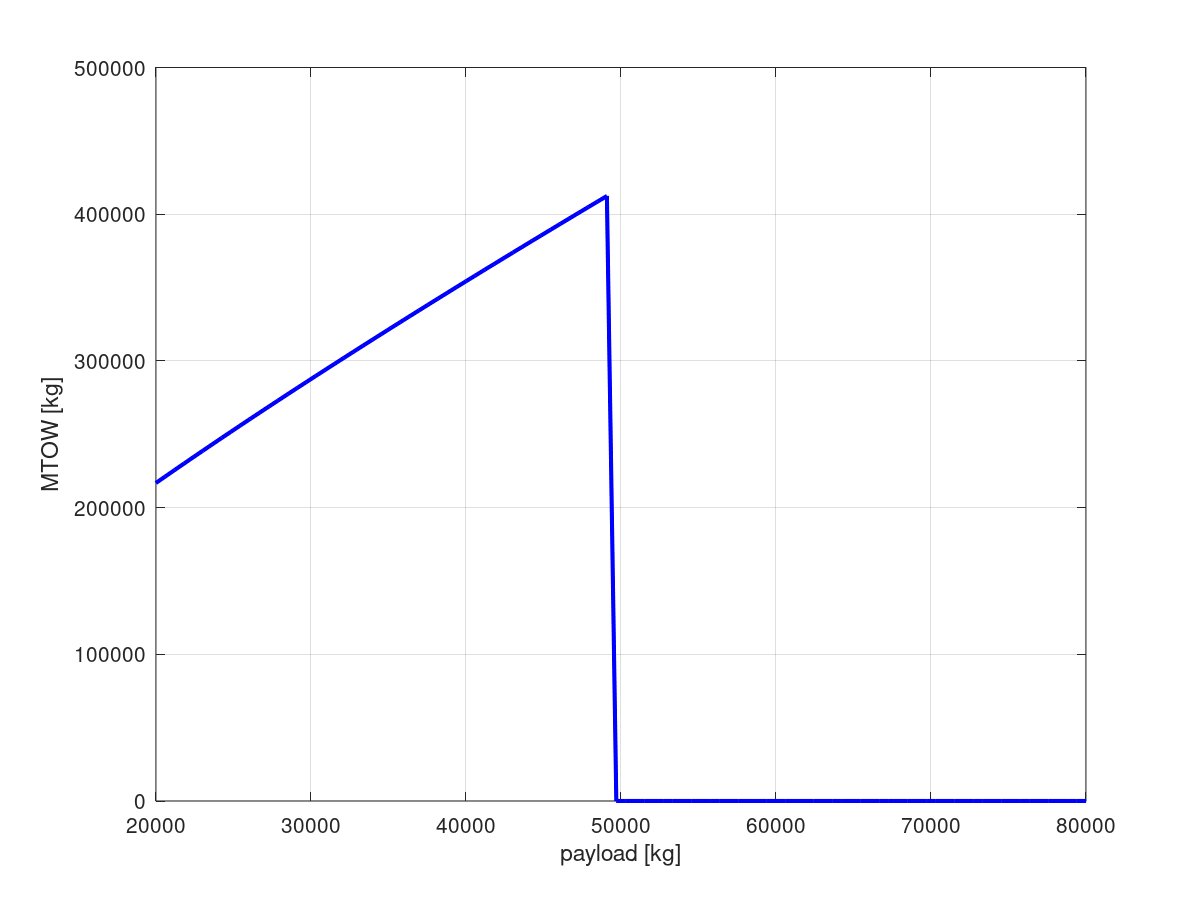
\includegraphics[width=\textwidth]{Sources/Plots_and_Pictures/MTOW_payload_2.png}
    \label{MTOW_Payload_15}
    \caption{MTOW-Payload (15000 km)}
\end{figure}
As you can see, there are areas where the function drops to a null value,
but that's because the MTOW ceases to have a physical meaning above or below certain
thresholds, depending on the input parameters. \\ 
However there seems to be a convergence slightly above 40 metric tonnes.
\clearpage

\section{Assignment 2\label{Assignment_2}}
\subsection{Assignment 2.1 and 2.2\label{Assignment_2.1}}
\textbf{Assignment:} Perform a Tradeoff and identify a suitable design point that 
guarantees the aircraft concept to be competitive with A350 and competitors. \\ \\ \\ 
\textbf{Assignment:} Create a Payload-Range Diagram representative of your aircraft concept. 
On the basis of the results achieved, draw different Payload-Range diagrams to explore 
the possibility to create a family concept.\\ \\ \\ 


Another key aspect to take into consideration is how the \textit{Payload} changes with 
 range, considering that fuel contribution to the total mass is obviously going
to change over time, thus influencing other factors as well. \\ 
The fuel volume of the Airbus A350 ($141 \ m^3$) as well as
the fuel itself (\textit{AVGAS}) have been taken as a reference point.\\ 
In order to better represent this function within a family of aircrafts that
is compatible with our statistical sample, a variation around the design point values has been 
taken into account.\\ 

\begin{itemize}
    \item Payload variation: $\pm \ 5000 \ kg$
    \item MTOW variation: $\left \{ {0.88 \ MTOW, 1.077 \ MTOW} \right \} \ kg$
    \item Range variation: $\pm \ 500 \ km$
\end{itemize}

The result is calculated and plotted with the function \autocite{Airbus_replacement_repo}
\begin{verbatim}
    payload_range_plotter.m
\end{verbatim}
which takes into consideration all the parameters involving the fuel, as well as other design values for the airplane.\\ 
The plotter can be called with input variations as many times as the user needs, while the `\textit{On}' parameter
is passed. \\ 
Finally, when the `\textit{Off}' parameter is passed, all the cases are plot on a single figure, with 
a randomized color palette.
\begin{figure}[h!]
    \phantomsection
    \centering
    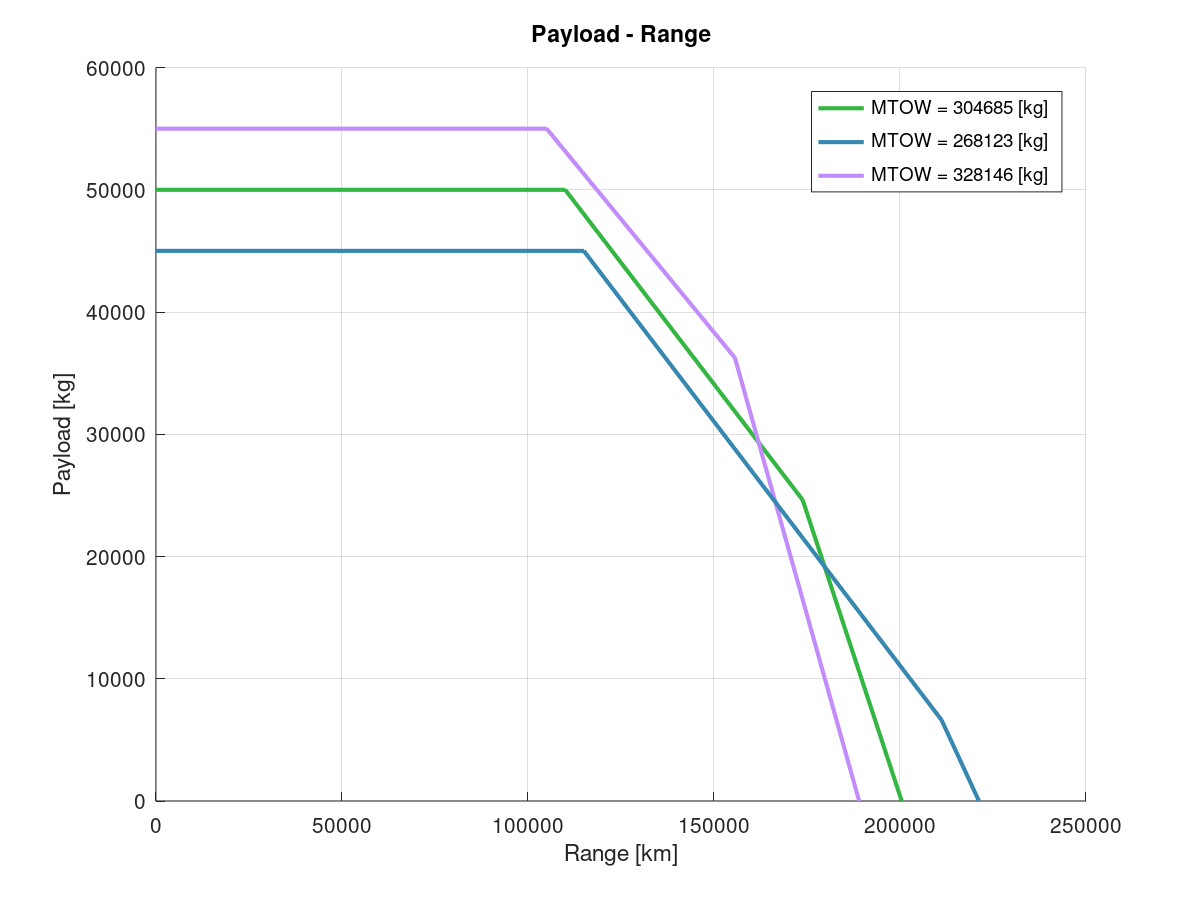
\includegraphics[width=\textwidth]{Sources/Plots_and_Pictures/Payload_range.png}
    \label{Payload_Range}
    \caption{Payload Range}
\end{figure}
\clearpage

As expected, the same fuel conditions for each sample case will produce the same slopes for each segment; moreover a higher
payload implies a higher MTOW (provided that all other factors are equalized), which in turn will reduce total range.\\ 
More precisely, the surface subtended by each segment defines three different areas (from left to right respectively) [\ref{Payload_Range}]:
\begin{itemize}
    \item Maximum payload
    \item Tradeoff between fuel and payload
    \item Tradeoff between payload and range
\end{itemize}

With a maximum design range of 15000 km and a starting payload of 50 metric tonnes, 
the designed aircraft is in an area where there needs to be a tradeoff between fuel and payload.\\ 
In order to achieve that range, some payload capacity needs to be sacrificed for more fuel.\\ 
However, with a minimum goal range of 11000 km, there is still is a chance to use the highest payload possible,
while increasing fuel, as that range falls within the first segment area. \\ 
It turns out that even the Airbus A350-900 XWB (which is the target retiring aircraft) declares
a maximum range of 15000 km; however, this range is not reached at maximum payload \autocite{Airbus_A350-900}.

\pagebreak
\subsection{Assignment 2.3\label{Assignment_2.3}}
\textbf{Assignment:} Once the maximum range requirement is refined,
 identify a set of city-pairs that can be connected with no-stop flight. \\ \\ \\ 
\pagebreak 

\subsection{Assignment 2.4\label{Assignment_2.4}}
\textbf{Assignment:} Build the Matching Chart for your case study and define
 Wing Surface and Engine Thrust \\ \\ \\ 

\pagebreak
\printbibliography
    
\end{document}

